% !TEX root = ../dissertation.tex

\chapter{Nonlinear Geometric Control}\label{sec:se3_control}

While there has been significant study of interplanetary transfer trajectories, relatively less analysis has been conducted on operations in the vicinity of asteroids.
The dynamic environment around asteroids is strongly perturbed and challenging for analysis and mission operations~\cite{scheeres1994,scheeres2000}.
Due to their low mass, which results in a low gravitational attraction, asteroids may have irregular shapes and potentially chaotic spin states.
As a result, typical approaches of assuming a inverse square gravitational model are at best inaccurate and at worst do not capture the true dynamic environment.
In addition, the vast majority of asteroid are difficult to track or measure using current ground-based optical sensors. 
Due to their small size, frequently less than \SI{1}{\kilo\meter}, and low albedo the reflected energy of these asteroids is insufficient for reliable detection or tracking.
Therefore, the dynamic model of the asteroid is relatively coarse prior to arrival of a dedicated spacecraft in the vicinity. 
As a result, any spacecraft mission to an asteroid is dependent on a robust dynamic simulation and must incorporate the ability to deal with uncertain forces and environments.

% talk about the coupling between attitude and translational states
Furthermore, since the magnitude of the gravitational attraction is relatively small, non-gravitational effects, such as solar radiation pressure or third-body effects, become much more significant.
As a result, the orbital environment is generally quite complex and it is difficult to generate analytical insights.
One key consideration is the coupling between rotational and translational states around the asteroid.
The coupling is induced due to the different gravitational forces experienced on various parts of the spacecraft.
The effect of the gravitational coupling is related to the parameter \(\epsilon = \frac{r}{R_c}\), where \(r\) is the characteristic spacecraft length and \(R_c\) is the orbital radius~\cite{hughes2004}.
For Earth based missions, the orbital radius is several orders of magnitude larger than the spacecraft length and \(\epsilon\) is small.
As a result, the corresponding gravitational moment is weak and can be neglected. 
Therefore, the translational and rotational equations of motion become decoupled and can be considered separately, significantly simplifying the analysis. 
However, for operations around an asteroid the orbital radius is much smaller, which leads to much larger values of \(\epsilon\) and much larger influence of the rotational and translational coupling.
References~\cite{elmasri2005} and~\cite{sanyal2004} investigated the coupling of an elastic dumbbell spacecraft in orbit about a central body, but only considered the case of a spherically symmetric central body.
Furthermore, the spacecraft model is assumed to remain in a planar orbit.
As result, these developments are not directly applicable to motion about an asteroid, which experience highly non-keplerian dynamics.

% now talk about the specific challenges of asteroid landing. there are lots of trajectory design papers and several have considered landing trajectories
An additional layer of complexity is the design of landing trajectories on asteroids.
Beginning with the first landing of NEAR Shoemaker on asteroid 433 Eros, there has been a concerted effort to develop techniques and methodologies for asteroid landing~\cite{dunham2002, kubota2006}.
There is already considerable knowledge on the planetary landing problem~\cite{acikmese2007, meditch1964, ingoldby1978}.
While conceptually similar, the landing of spacecraft on small bodies requires additional consideration. 
The surface of an asteroid is highly irregular and, as discussed previously, there is a large coupling between the translational and rotational dynamics of the vehicle, which is further exaggerated when close to the surface.
References~\cite{guelman1994, furfaro2013, zexu2012} consider the soft landing problem on an asteroid.
These approaches were primarily based on nonlinear control techniques which allowed for the development of closed loop controllers which enable landing.
However, only the translational dynamics of the body was considered and no notion of the attitude dynamics or it's coupling to the position is considered.
Furthermore, relatively simple gravitational models are used which make the results unsuitable for operations near irregular bodies.
In this chapter, we derive and develop a nonlinear geometric controller for the coupled dynamics of a spacecraft around an asteroid.

An additional layer of complexity is the design of landing trajectories on asteroids.
Beginning with the first landing of NEAR Shoemaker on asteroid 433 Eros, there has been a concerted effort to develop techniques and methodologies for asteroid landing~\cite{dunham2002, kubota2006}.
There is already considerable knowledge on the planetary landing problem~\cite{acikmese2007, meditch1964, ingoldby1978}.
While conceptually similar, the landing of spacecraft on small bodies requires additional consideration. 
The surface of an asteroid is highly irregular and, as discussed previously, there is a large coupling between the translational and rotational dynamics of the vehicle, which is further exaggerated when close to the surface.
References~\cite{guelman1994, furfaro2013, zexu2012} consider the soft landing problem on an asteroid.
These approaches were primarily based on nonlinear control techniques which allowed for the development of closed loop controllers which enable landing.
However, only the translational dynamics of the body was considered and no notion of the attitude dynamics or it's coupling to the position is considered.
Furthermore, relatively simple gravitational models are used which make the results unsuitable for operations near irregular bodies.
\section{Geometric Control}

A wide variety of control schemes have been proposed for asteroid landing missions~\cite{furfaro2013,li2011a}.
In addition, there are a  variety of controllers developed for systems evolving on \( \SE \)~\cite{lee2010,lee2013}.
In this paper, we extend their use from quadrotor aerial vehicles into the space domain. 
This approach addresses many of the issues associated with the related work on asteroid landings.
The geometric control methods used to develop these nonlinear controllers allow for the development of control systems for dynamic systems which evolve on nonlinear manifolds. 
By developing the control system directly on the nonlinear manifold, geometric control techniques provide unique advantages as compared to those developed using local coordinate representations.
Furthermore, the geometric controller avoids the chattering issues inherent in the previous sliding mode control approaches to asteroid landing.
In addition, rather than offering only a bounded stability guarantee, the proposed nonlinear geometric controller guarantees almost global tracking of the attitude and translational states. 
This stability guarantee is critical for mission operations passing close to the surface over highly irregular terrain.
Furthermore, the coupled geometric controller explicitly considers the attitude coupling of the body in contrast to many of the previous approaches.
We briefly summarize the key developments of the \( \SE \) control scheme and leave the detailed derivations to the source manuscripts~\cite{lee2010,lee2013}.
% TODO Basics of geometric control

% TODO Derive attitude and translation control seperately

% TODO Specifics for use in the asteroid case

\subsection{Spacecraft Dynamic Model}\label{sec:controlled_dynamic_model}
We consider the controlled motion of a rigid dumbbell spacecraft about a small body.
% TODO Add some citations for dumbbell for use in spacecraft
The dumbbell spacecraft consists of two masses connected by a massless rod and is a well-known representation of a multi body spacecraft.
Furthermore, the dumbbell model captures the important interactions of the coupling between orbital and attitude dynamics. 
As a result, this simple model is useful to capture the main characteristics of a wide variety of spacecraft configurations.
Typically, spacecraft have mass concentrated in a central structure, referred to as the bus, which houses the command and control system, actuators, fuel, sensors etc. 
In addition, comparatively light-weight solar panels extend from the bus to provide electrical energy from solar radiation. 
As a result, the distributed mass of the spacecraft is captured with the dumbbell representation.
In this section, we briefly review the polyhedron potential model and then present the derivation of the coupled dynamics of a dumbbell spacecraft about an asteroid.
In this work, we assume that the asteroid is much more massive than the spacecraft and its motion is not affected by that of the spacecraft.
This assumption allows us to treat the motion of the vehicle independently from that of the asteroid, instead of treating the more complicated full-body problem. 
% TODO Add link to dynamic model given in previous section
% The spacecraft model is the same as that defined in 

In this section, we develop a coupled control system to track a desired trajectory.
We assume that the desired trajectory, \( R_d(t), \vb{x}_d(t) \), are defined as the rotation matrix of the spacecraft body frame with respect to the inertial frame and the relative position of the spacecraft center of mass with respect to the asteorid and defined in the inertial frame, respectively.
In contrast to controller derived for quadrotor \gls{uav}, the attitude and translational motion is only lightly coupled in the spacecraft scenario.
From the dynamic equations of motion, the coupling between the translational and rotational dynamics is due to the gravitational moment on the spacecraft.
Furthermore, we assume that we have a fully actuated spacecraft such that we can apply a torque about all three rotational axes and a force in all three directions.
This is in contrast to \glspl{uav} where the system is underactuated and in order to produce certain translational forces the system must first rotate.
This is a relatively standard assumption in the astrodynamics community as most spacecraft contain seperate systems for attitude control, e.g. \glspl{rwa}, \glspl{cmg}, or cold gas thrusters, and translational control, e.g. cold-gas thrusters, electric propulsion, or large chemical rockets~\cite{hughes2004,wertz1978}.
However, there are also many examples of underactuated spacecraft, such as those with damaged components~\cite{petersen2015a} or cubesats with limited cost and/or size budgets.
% TODO Add citaitons for these papers
In these situations, there are a variety of methods to handle the underactuation, ranging from optimal control techniques, exploiting external forces, or utilizing multiple control loops.


\subsection{Attitude Control}
In order to determine the attitude control input, we first define a desired attitude tracking command.
An arbitrary smooth attitude tracking command \( R_d (t) \in \SO \) is given as a function of time.
The corresponding angular velocity command is obtained using the attitude kinematics equation, \( \hat{\Omega}_d = R_d^T \dot{R}_d \).
With the desired attitude command, we then define the errors associated with the attitude and angular velocity.
The attitude and angular velocity tracking errors must be careful chosen to remain on the tangent bundle of \SO.
First, an attitude error function is defined on \( \SO \times \SO \) as
\begin{align}\label{eq:attitude_error_function}
    \Psi(R, R_d) = \frac{1}{2} \tr{I - R_d^T R}.
\end{align}
This positive definite function parameterizes the error between the current attitude, \( R \), and the desired attitude command \( R_d \).
Using the variations of \( \Psi \) gives the attitude tracking error vector \( e_R \in \R^3 \) as
\begin{align}\label{eq:attitude_error_vector}
    e_R = \frac{1}{2} \parenth{R_d^T R - R^T R_d^\vee}.
\end{align}
After further manipulation and using the attitude kinematics equation from~\cref{eq:attitude_kinematics}, it is possible to define the angular veloicty tracking error \( e_\Omega \in \R^3 \) as
\begin{align}\label{eq:angular_velocity_error_vector}
    e_\Omega = \Omega - R^T R_d \Omega_d .
\end{align}
With the properly defined attitude error vectors the rotational control input is defined as 
\begin{align*}\label{eq:rotational_control}
    \vb{u}_m = - k_R e_R - k_\Omega e_\Omega + \Omega \times J \Omega - J \parenth{\hat{\Omega} R^T R_d \Omega_d - R^T R_d \dot{\Omega}_d} - \vb{M}_1 - \vb{M_2} 
\end{align*}
where \( k_R, k_\Omega \) are positive controller constants.

\subsection{Translation Control}
The translational control input is defined in a similar manner. 
First we define a smooth tracking command \( x_d(t) \in \R^3 \), which defines the desired position of the spacecraft in the inertial frame.
The tracking error vectors are easier to define as they evolve on a Euclidean space rather than a nonlinear manifold and are given by
\begin{align}
    e_x = x - x_d ,\\
    e_v = v - \dot{x}_d .
\end{align}
With the error variables, the translational control input is then given by
\begin{align}\label{eq:translation_control}
    \vb{u}_f = - k_x e_x  - k_v e_v + ( m_1  + m_2 ) \ddot{x}_d - \vb{F}_1 - \vb{F}_2 ,
\end{align}
where \( k_x, k_v \) are positive constants. 
The control gains are chosen based on the desired closed-loop system response. 
A variety of techniques are available to choose these gains, but a simple linear analysis offers a straightforward and systematic approach to choosing suitable values. 
We use the control inputs defined in~\cref{eq:translation_control,eq:rotational_control} and substitute them into the dynamic equations of motion in~\cref{eq:translational_dynamics,eq:attitude_dynamics}.
This results in the dynamics of the error variables and the gains are chosen to ensure the error behavior meets desired performance criteria, such as percent overshoot or settling time~\cite{nise2004}.


\section{Numerical Example}

% TODO Disucss numerical implementation
Typically, spacecraft missions require extensive interaction from ground based human operators. 
This interaction ranges from system health checks to navigation and hardware commands.
In addition, there is frequently a large group of analysts in support of any given mission. 
A wide variety of factors make human in the loop control of spacecraft especially difficult.
First, the vast distances cause significant time delays which render it impossible to react immediately to events experienced by the spacecraft. 
Furthermore, deep space missions are designed for continuous mission operations for many years or even decades. 
It is becoming increasingly difficult to maintain trained and knowledgeable staff for several decades in order to support a single mission.
In addition, these operators become increasingly scarce as the contemporary hardware and software tools surpass those of these decades old spacecraft. 
As a result, there is a large focus on completely autonomous spacecraft systems.

We present a numerical simulation of a rigid dumbbell about asteroid Itokawa.
The dumbbell spacecraft is composed of two equal masses, \( m_1, m_2 = \SI{500}{\kilo\gram} \), seperated by \( l = \SI{3}{\meter} \).
The dumbbell body frame is defined with the first body fixed axis, \( \vb{b}_1 \), originating at the center of mass of the spacecraft and directed along the vector from \( m_1 \) towards \( m_2 \).
The other two axes of the spacecraft fixed frame are chosen orthogonal to the \( \vb{b}_1 \) and lie in the plane orthogonal to the dumbbell axis of symmetry. 
A camera, using the parameters from~\cref{tab:camera_parameters}, is aligned with the \( \vb{b}_1 \) axis and used to feed image data to the ORB-SLAM system.
A numerical simulation is used to demonstrate the geometric control of the coupled motion of the spacecraft, and the ability to estimate the motion of the spacecraft from monocular imagery.

The initial condition of the spacecraft is defined as
\begin{align}
    \vb{x}_0 &= \begin{bmatrix} 0 & -2.550 & 0 \end{bmatrix} \si{\kilo\meter}, \\
    R_0 &= \exp { \frac{\pi}{2} \vb{e}_3 } .
\end{align}
The spacecraft begins on the inertial \( \vb{e}_2 \) axis and initially pointing at the asteroid. 
A tracking command is designed to transition the spacecraft towards the asteroid fixed \( \vb{f}_1  \) axis followed by a vertical descent along towards the asteroid surface.
The translational command is divided into two stages, a traverse step where the spacecraft follows a trajectory to align itself with the \( \vb{f}_1 \) axis and a landing step where the spacecraft follows a constant velocity descent towards the surface. 
The desired position command is defined as
\begin{align}
    \vb{x}_d = 
    \begin{cases}
        2.550 \begin{bmatrix} \sin{\omega t} & -\cos{\omega t} & 0 \end{bmatrix}, & t \leq t_d \\
        R_A \begin{bmatrix} \frac{2}{t_d} (t - t_d) + 2.550 & 0 & 0 \end{bmatrix}, & t > t_d , 
    \end{cases}
\end{align}
where \( \omega = \frac{\pi}{2 t_d} \), \( t_d \) is the time from the simulation start when the constant velocity descent should begin, and \( t \) is the simulation time step.

The desired attitude command is chosen such that the spacecraft camera axis, \( \vb{b}_1 \), is directed along the nadir towards the asteroid.
It is sufficient to define two orthogonal vectors to uniquely determine the attitude of the spacecraft.
The \( \vb{b}_{3d} \) vector is chosen to lie in the plane spanned by \(\vb{b}_{1d} \) and \( \vb{e}_3 = \vb{f}_3 \).
The desired attitude command is defined as
\begin{align}
    \vb{b}_{1d} &= - \frac{\vb{x}}{\norm{\vb{x}}} , \\
    \vb{b}_{3d} &= \frac{\vb{f}_3 - \parenth{\vb{f}_3 \cdot \vb{b}_{1d}} \vb{b}_{1d}}{\norm{\vb{f}_3 - \parenth{\vb{f}_3 \cdot \vb{b}_{1d}} \vb{b}_{1d}}}, \\
    \vb{b}_{2d} &= \vb{b}_{3d} \times \vb{b}_{1d} , \\
R_d &= \begin{bmatrix} \vb{b}_{1d} & \vb{b}_{2d} & \vb{b}_{3d} \end{bmatrix} .
\end{align}
The camera axis is aligned with the spacecraft \( \vb{b}_ 1 \) axis, which is direted towards the asteroid, throughout the landing trajectory as the spacecraft moves in the equatorial plane of the asteroid.

The simulation is carried out over \SI{7200}{\second} with the spacecraft following a circular trajectory for the first \SI{3600}{\sec} before vertically descending in the body fixed frame for the last \SI{3600}{\second}.
\Cref{fig:true_landing_trajectory} shows a view from the positive \( \vb{f}_3 \) pole of the asteroid of the simulated trajectory. 
The position of the center of mass of the dumbbell is shown in blue, while the pointing direction of the camera axis is defined in red. 
The attitude of the dumbbell is displayed at several points along the trajectory demonstraiting the pointing of the camera. 
Furthermore, asteroid Itokawa is shown in its final orientation at the completion of the landing simulation. 
\Cref{fig:pos_components} shows that the nonlinear controller is able to accurately track the desired translational trajectory for the duration of the simulation.
\begin{figure}[htbp]
    \captionsetup[subfigure]{position=b}
    \centering
    \subcaptionbox{Planar view of landing trajectory\label{fig:true_landing_trajectory}}{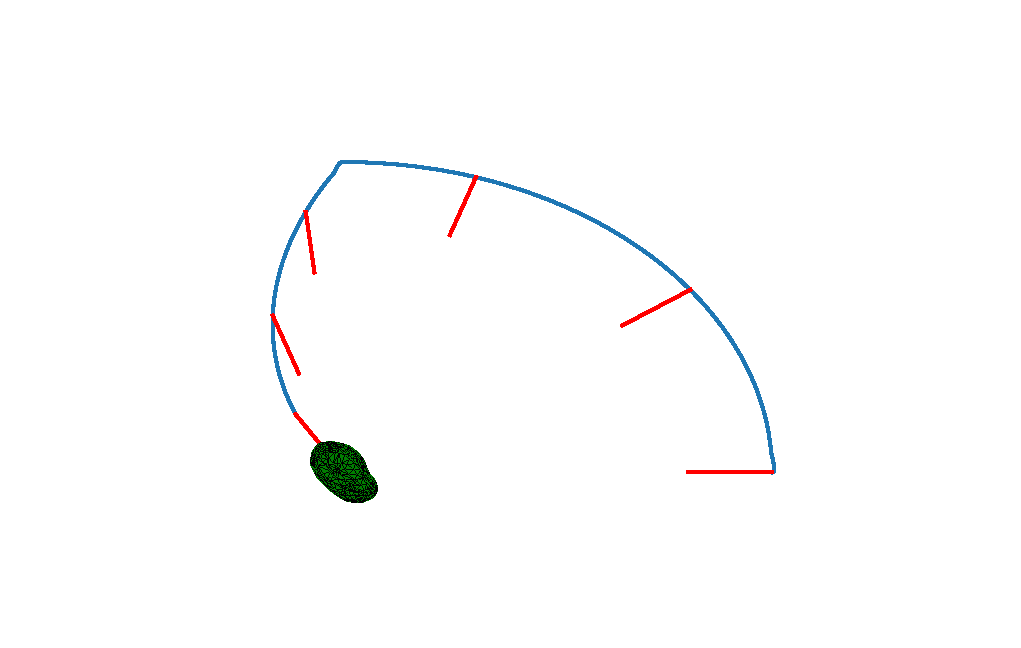
\includegraphics[width=0.5\textwidth]{figures/2017_AAS_fall/traj_fig.pdf}}~
    \subcaptionbox{Position of spacecraft in the inertial frame\label{fig:pos_components}}{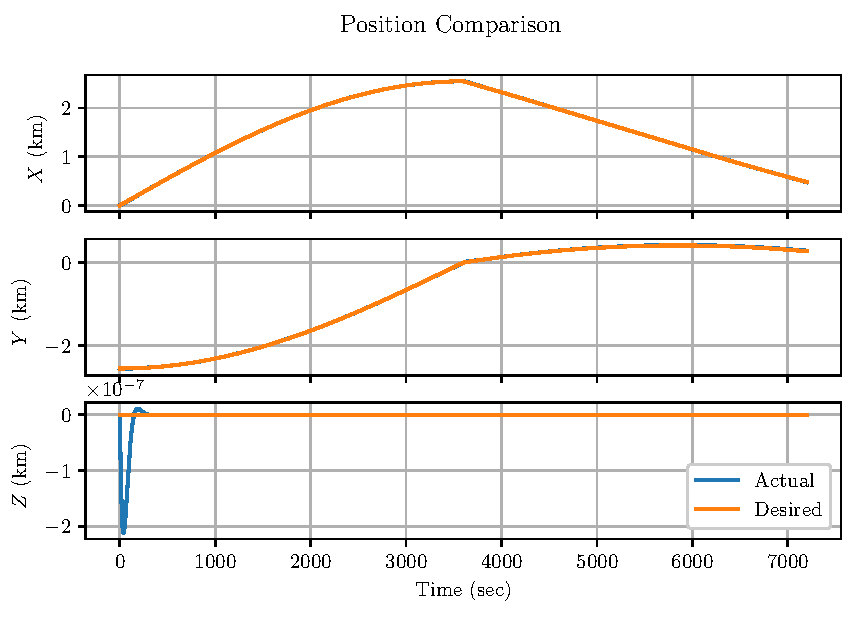
\includegraphics[width=0.5\textwidth]{figures/2017_AAS_fall/pos_fig.pdf}}
    \caption{Landing trajectory to asteroid Itokawa~\label{fig:position}}
\end{figure}
